\clearpage
\subsection*{\texttt{ex8a\_L7\_periodic}}
Initial deviation $z(0)$ (radians for angles, SI units otherwise):
\begin{center}\scriptsize\texttt{[0.003138205, 0.01745329, -0.009800946, -1.197667e-19, 7.378286e-18, -2.67647e-18]}\end{center}
$x^e=[0,0,0,0,0,0]^T$, $x(0)=x^e+z(0)$.
The initial state is selected numerically from an eigenmode; see the source code. Linear states are deviations from equilibrium.
\begin{figure}[!ht]
\centering
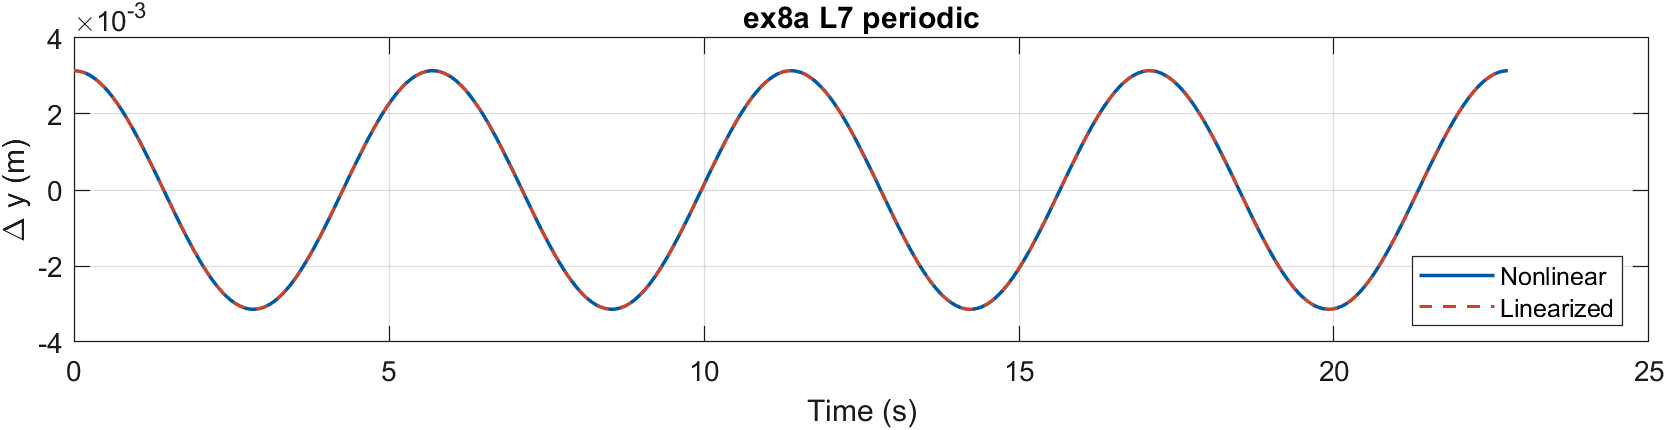
\includegraphics[width=0.94\linewidth]{figures/ex8a_L7_periodic_y.png}
\caption{$\Delta y$: nonlinear and linearized time histories.}
\end{figure}
\begin{figure}[!ht]
\centering
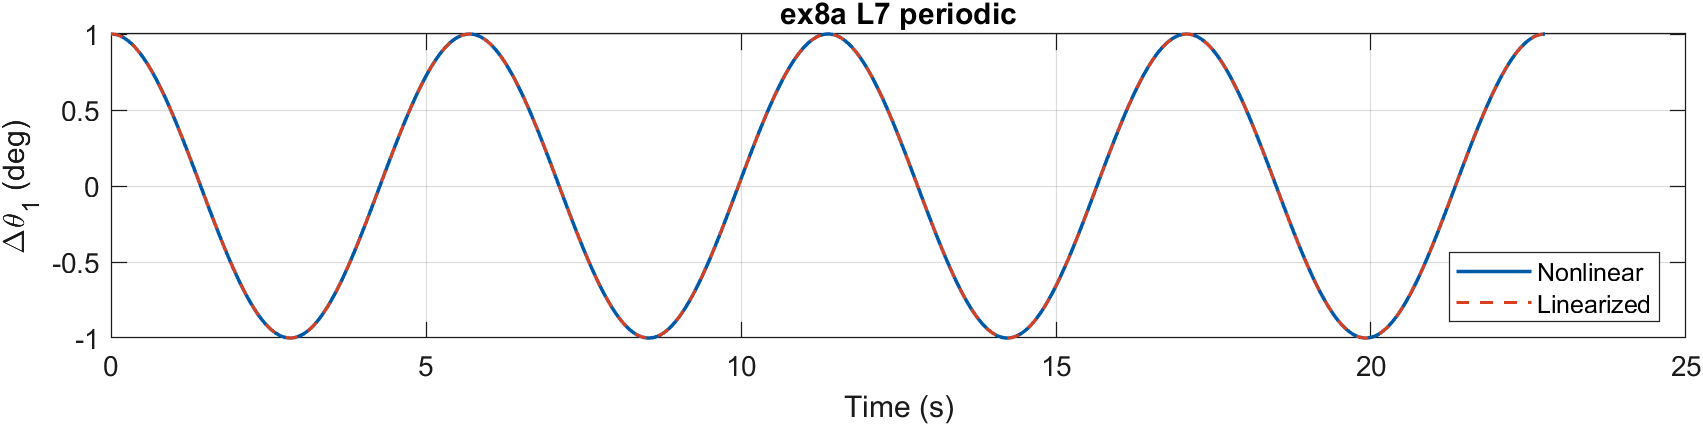
\includegraphics[width=0.94\linewidth]{figures/ex8a_L7_periodic_theta1.png}
\caption{$\Delta\theta_1$: nonlinear and linearized time histories.}
\end{figure}
\begin{figure}[!ht]
\centering
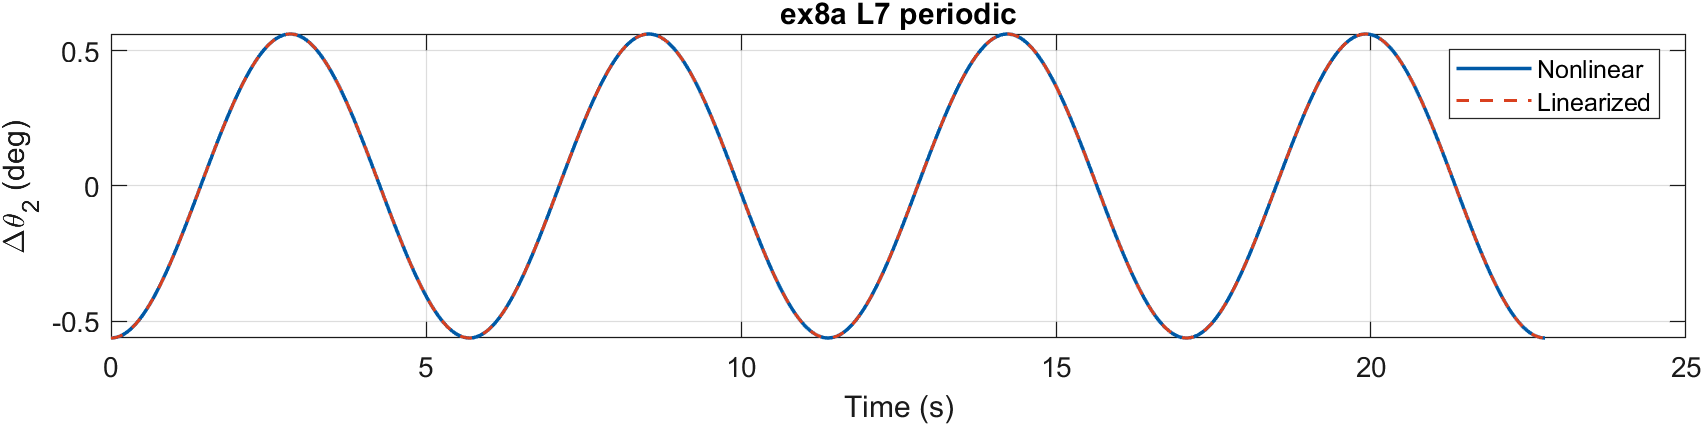
\includegraphics[width=0.94\linewidth]{figures/ex8a_L7_periodic_theta2.png}
\caption{$\Delta\theta_2$: nonlinear and linearized time histories.}
\end{figure}
